% !TeX root = ../main.tex

\chapter[Introduction to be shown in ToC] % chapter name to be shown in ToC
        {Introduction}
\label{chp:Introduction}
\chaptermark{Introduction header} % chapter name to be shown in header

This is a template for NTU thesis. See some notes on usage of 
references in Sec.~\ref{sec:ref}, compilation (Sec.~\ref{sec:com}) and figures (Sec.~\ref{sec:fig}). 

\section{References}
\label{sec:ref}

Use \hologo{BibTeX} for references. The references should be written into {\tt back\textbackslash reference.bib}, and the 
The format of each reference in the {\tt reference.bib} is directly provided by inSPIRE, clicking on the \hologo{BibTeX} link. 

In the bibliography example file the Belle II TDR~\cite{Abe:2010sj} reference is included, as well as 
the \textsc{Geant 4}~\cite{Agostinelli:2002hh} and the physics case paper~\cite{Aushev:2010bq} references.

\section{Compiling}
\label{sec:com}

This template requires \hologo{XeLaTeX} to compile.

\section{Figures}
\label{sec:fig}

Figures are included as usually, shown in the example of Fig.~\ref{fig:belledetector} below. Beside the pdf also jpg and eps 
formats can be used. Specifiy the figure files in \\
{\tt
\textbackslash includegraphics[width=0.5\textbackslash textwidth]\{path\_to\_figure.pdf\}\\
}
without extensions ({\tt pdflatex} command will take care of that, by using {\tt epstopdf} package 
for the eps files, for example). 

If you use Overleaf to compile, it is recommended to use pdf file instead of others.

\begin{figure}
\begin{center}
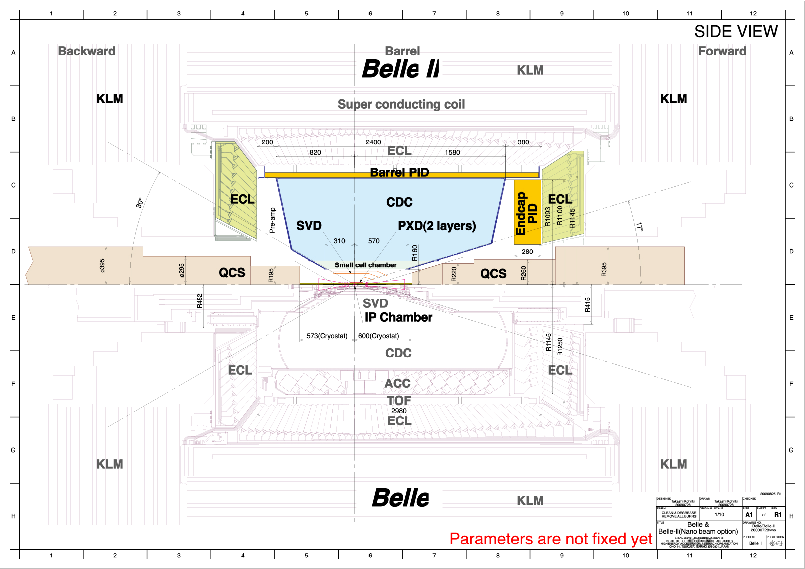
\includegraphics[width=0.5\textwidth]{figures/belle2detector.pdf}
  \caption[Belle II detector to be shown in List of Figure.]{Belle II detector configuration. Get from TDR~\cite{Abe:2010sj}.}
  \label{fig:belledetector}
\end{center}
\end{figure}

If you want to use captions for subfigure in one figure environment, you can use subfigure package as in Fig.~\ref{fig:NTUlogo}.

\begin{figure}[ht]
\centering
    \begin{subfigure}[b]{0.3\textwidth}
        
\includegraphics[width=\textwidth]{figures/NTU_logo_color.pdf}
        \caption{Colored logo.}
    \end{subfigure}
    \hspace{0.2\textwidth}
    \begin{subfigure}[b]{0.3\textwidth}
        
\includegraphics[width=\textwidth]{figures/NTU_logo_gray.pdf}
        \caption{Gray logo.}
    \end{subfigure}
\caption{NTU logo.}
\label{fig:NTUlogo}
\end{figure}

If you are creating figures from {\tt ROOT}, your are advised to use the Belle2 style files from my \href{http://hep5.phys.ntu.edu.tw/indico/event/1174/contribution/8/material/slides/0.pdf}{plotting style workshop}.

\clearpage

\section{Tables}
\label{sec:tab}

A table can be constructed by {\tt tabularx} environment. There are three newly defined column type in this template:\\
{\tt C}: equally share the column width and automatically change line in the text, with center text alignment.\\
{\tt L}: equally share the column width and automatically change line in the text, with left text alignment.\\
{\tt R}: equally share the column width and automatically change line in the text, with right text alignment.

\begin{table}[ht]
\begin{center}
\begin{tabularx}{\textwidth}{c|L|CR}
\hline \hline
This column not sharing width & This column sharing width and automatically change line & This column sharing width and automatically change line &  This column sharing width and automatically change line  \\
\hline 
some table content & \multirow{2}{*}{multirow} & \multicolumn{2}{c}{$M_{bc}=5.29~\text{GeV}/c^2$}    \\
\cline{3-4}
other table content &  & content with \newline line change\gape{\footnotemark} & $-\pi\textnormal{--}-\frac{\pi}{2}$ \\
\hline \hline
\end{tabularx} 
\caption{A simple table contains different contents.}
\label{tab:tab}
\end{center}
\end{table}

\footnotetext{Set footnote like this if you want to add it in a table.}

\section{Equation}

If you want to write some equations in your thesis, you can use {\tt equation} environment, as shown in Eq.~\ref{eqn:eqn} --~\ref{eqn:eqn2}.

\begin{equation}
f(x)=\left\{
\begin{array}{l}
v_{0} + 2\sum\limits_{n=1}^\infty v_{n}\cos{(nx)}, \\
\sum\limits_{n=0}^\infty a_{n}(x)^n + a_{4} \cos{(2x)}, \\
\sum\limits_{n=0}^\infty a_{n}(x)^n.
\end{array} \right.
\label{eqn:eqn}
\end{equation}

\begin{equation}
\begin{aligned}
\int L \text{d}t = &  300~\rm fb^{-1}, \\
% column1 & column2 \\
\int L \text{d}t = &  8\times10^{35}~\text{cm}^{-2} \text{s}^{-1}. 
\end{aligned}
\label{eqn:eqn2}
\end{equation}

Remember that an equation is also included in your paragraph, so don't do extra line break when input an {\tt equation}. For example, this is an equation to be described within a sentence, written as
\begin{equation}
f(\xi)=\xi(\Vec{a}\times\Vec{b})\cdot\Vec{c},
\label{eqn:eqn3}
\end{equation}
and the sentence behind it is not indented. There is a comma behind the equation to claim that there are still some words. For very short equation or math notation, you can directly describe it in line, such as $\Delta E< 0.01~\text{MeV}$ or $p_{\rm T} \ge 0.25~\text{GeV}/c$.